\documentclass[a4paper]{article}
\usepackage{WUST-AAE-NMaO-Report}
\usepackage{amsfonts}
\usepackage{amsmath}
\usepackage[polish,main=english]{babel}
\usepackage{indentfirst}
\usepackage{nameref}
\usepackage{natbib}
\usepackage{listings}
\usepackage{matlab-prettifier}
\usepackage{pdfpages}
\usepackage{pgfplots}
\usepackage{systeme}
\usepackage{tasks}
\usepackage{todonotes}

% \usepackage{amssymb}
% \usepackage{titlesec}
% \usepackage{vmargin}
% \usepackage{fancyhdr}
% \usepackage{xcolor}
% \usepackage{multicol}


\usepackage{float} 
\usepackage{graphicx,xcolor,colortbl}    
\usepackage{epstopdf,epsfig}   


%%%%%%%%%%%%%%%%%%%%%%%%%%%%%%%%%%%%%%%

\title{Numerical Methods and Optimization Report 3:
Ill-posed least-squares problems}
\author{Kamil Czop 259613\\Sergiusz Warga 230757}
\reporttutor{dr hab.\ inż. Rafał Zdunek}

\begin{document}

\maketitle
\tableofcontents
\listoftodos
\pagebreak

\section{Problems}
\subsection{Problem 1}%
\label{sec:problem_1}
Find the solution that best approximates the system of inconsistent linear equations:
\begin{tasks}(3)
  \task $\systeme{3x_1-x_2=4,x_1+2x_2=0,2x_1+x_2=1}$
  \task $\systeme{3x_1+x_2+x_3=6,
  2x_1+3x_2-x_3=1,
  2x_1-x_2+x_3=0,
  3x_1-3x_2+3x_3=8}$
  \task $\systeme{x_1+x_2-x_3=5,
  2x_1-x_2+6x_3=1,
  -x_1+4x_2+x_3=0,
  3x_1+2x_2-x_3=6}$
\end{tasks}
%%%%%%%%%%%%%%%%%%%%%%%%%%%%%%%%%%%%%%%%%%%%%%%%%%%%%%%%%%%%%%%%%%%%%%%%%%%%%%%
\subsubsection*{Mathematics}
%%%%%%%%%%%%%%%%%%%%%%%%%%%%%%%%%%%%%%%%%%%%%%%%%%%%%%%%%%%%%%%%%%%%%%%%%%%%%%%
The system of inconsistent linear equations comprises linearly independent equations,
whose number is greater than the number of unknown variables.
Such a system may be expressed in the form:
\begin{equation*}
  \matr{Ax}=\matr{b}, \quad \text{where} \quad
  \matr{A}\in\mathfrak{R}^{m\times{}n}, \quad
  \matr{b}\in\mathfrak{R}^m, \quad
  \matr{x}\in\mathfrak{R}^n, \quad \text{and} \quad m\geq{}n
\end{equation*}
and has no solution. We may attempt to find the best approximate solution to such a
system by solving the minimization problem:
\begin{equation*}
  \min_{\matr{x}}{\left\lVert\matr{b}-\matr{A}\matr{x}\right\rVert}_2
\end{equation*}
For such a system, an associated system of \textit{normal equations} is defined to be:
\begin{equation}
  \matr{A}^T\matr{Ax}=\matr{A}^T\matr{b}
\end{equation}
which is always consistent.
The solution has the form:
\begin{equation}
  \label{eq:normal_approximation}
  \matr{x}=\left(\matr{A}^T\matr{A}\right)^{-1}\matr{A}^T\matr{b}
\end{equation}
%%%%%%%%%%%%%%%%%%%%%%%%%%%%%%%%%%%%%%%%%%%%%%%%%%%%%%%%%%%%%%%%%%%%%%%%%%%%%%%
\subsubsection*{Solution}
%%%%%%%%%%%%%%%%%%%%%%%%%%%%%%%%%%%%%%%%%%%%%%%%%%%%%%%%%%%%%%%%%%%%%%%%%%%%%%%
The solutions to all the systems of linear equations above may be easily approximated
with the \MATLAB{} function implementing~\eqref{eq:normal_approximation}:
\lstinputlisting[style=Matlab-editor]{problems/normal_approximation.m}
Then, the solution may be verified with \lstinline[style=Matlab-editor]{x - A\b}:
\lstinputlisting[style=Matlab-editor]{problems/Problem_1.m}

\subsection{Problem 2}%
\label{sec:problem_2}
Compute the largest and the smallest eigenvalue to the following matrix, using the
scaled power algorithm and the shifted inverse power algorithm, respectively:
\begin{equation*}
    \matr{A} = 
    \begin{bmatrix}
        4 & 2 & 0 & 0 \\
        1 & 4 & 1 & 0 \\
        0 & 1 & 4 & 1 \\
        0 & 0 & 2 & 4
    \end{bmatrix}
\end{equation*}
%%%%%%%%%%%%%%%%%%%%%%%%%%%%%%%%%%%%%%%%%%%%%%%%%%%%%%%%%%%%%%%%%%%%%%%%%%%%%%%
\subsubsection*{Mathematics}
%%%%%%%%%%%%%%%%%%%%%%%%%%%%%%%%%%%%%%%%%%%%%%%%%%%%%%%%%%%%%%%%%%%%%%%%%%%%%%%
Basing on information included in ~\cite{Zdunek}, methods that allow for finding eigenpairs are \textit{Power method} 
(in sources such as refered as \textit{Power iteration}) and \textit{shifted inverse power method}, (Also known as \textit{inverse iteration}\cite{Demmel}).\\
\\
Power iteration allows for quick and easy computation of dominant eigenvalue and coresponding eigenvector $(\lambda_1, x_1)$ of diagonalizable matrix 
\textbf{A}$\in \mathfrak{R}^{n_xn}$ where eigenvalues are in following sequence $|\lambda_1| > |\lambda_2| > ... > |\lambda_n|$.
Initial condition for power method requires random vector that is approximation of dominant eigenvector, which is symbolized as $\xi_0$. Vector generated as such is then immediately which is also normalized in the same step 
\begin{equation*}
    \xi_0 = \frac{\xi_0}{||\xi_0||_2} 
\end{equation*}
This step is done to prevent problems with approximation, underflow, overflows and hold the convergence criterion, it helps at making successive approximations of the eigenvector where normalization helps the randomly generated vector focus on the direction rather than magnitude, reducing algorithm runtime allowing for faster honing to direction of dominant vector.\\
Power iteration as name suggests is iterative technique which computes the result in each loop iteration.
Update formula is similar to initial vector normalization taking into calculation base matrix on which we are trying to define dominant eigenvector
\begin{equation*}
    \xi_k = \frac{A \xi_{k-1}}{||A \xi_{k-1}||_2}
\end{equation*}
Each loop step hones closer to the direction of dominant eigenvector. Because of iterative nature of algorithm, we can break out of the loop after certain amount of steps or after we reach threshold convergence rate $\epsilon$, which is calculated by normalizing the difference between $\xi_k$ and $\xi_{k-1}$.
\begin{equation*}
    ||\xi_k - \xi_{k-1}|| < \epsilon
\end{equation*}
As a final step of power method we need to extract our dominant eigenpair. 
Method for obtaining approximation of our dominant eigenvector is taking last $\xi_k$.\\
Obtaining eigenvalue is bit more complex
\begin{equation*}
    \lambda_1 \approx \xi_k^T A \xi_k 
\end{equation*}
\\
One of biggest disadvantages of Power method is that it can only determine dominant eigenpair, for finding other eigenpairs we need to use more complex variation which is Inverse iteration.
Inverse power method allows for finding any eigenpair, by variable $\sigma$ also known as shift\cite{Demmel}.
Specified $\sigma$ value allows us to converge to the closest eigenvalue to shift rather than only $\lambda_1$. Further steps in loop deviate slightly from Power method, steps that update our next $\xi_k$, we no longer multiply A by previous $\xi_{i-1}$. This calculation also takes in consideration shift modifying formula for next $\xi$ as such:
\begin{equation*}
    \begin{matrix}
        y = (A - \sigma I)^-1 \xi_{i-1}\\
        \xi_i = \frac{y}{||y||_2}
    \end{matrix}
\end{equation*}
Further steps stay consistent with Power method.

\subsubsection*{Solution}
Script that plots and displays results from both methods used accordingly to it's specific task:
\lstinputlisting[style=Matlab-editor]{problems/Codes/Problem_2/main.m}

Running MATLAB script yields such results:
\lstinputlisting[style=Matlab-editor]{problems/Results/Problem_2.m}

\begin{figure}[H]
    \centering
    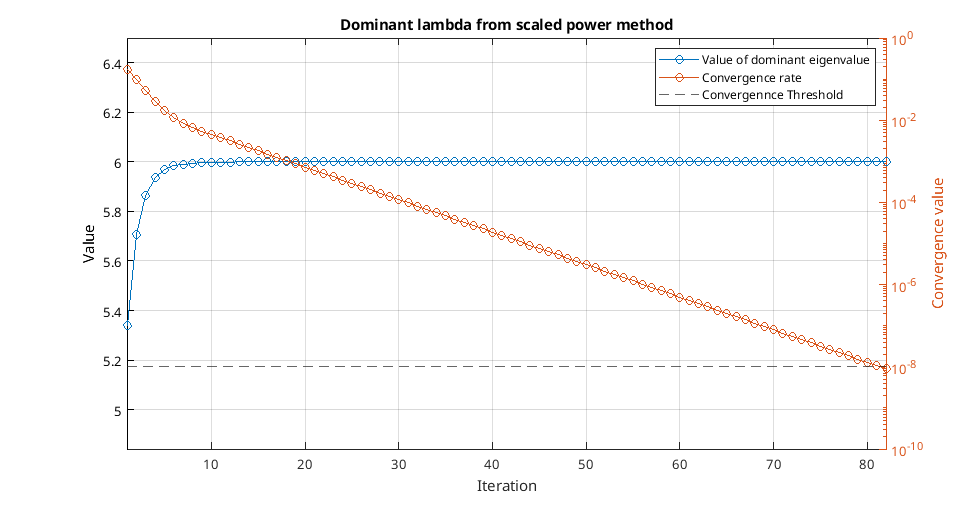
\includegraphics[width=1\textwidth]{problems/Figures/Problem2ScaledPowerMethod.png}
    \caption{Eigenvalue approximation and convergence rate over each iteration of power method.}
    \label{fig:Power}
\end{figure}

\begin{figure}[H]
    \centering
    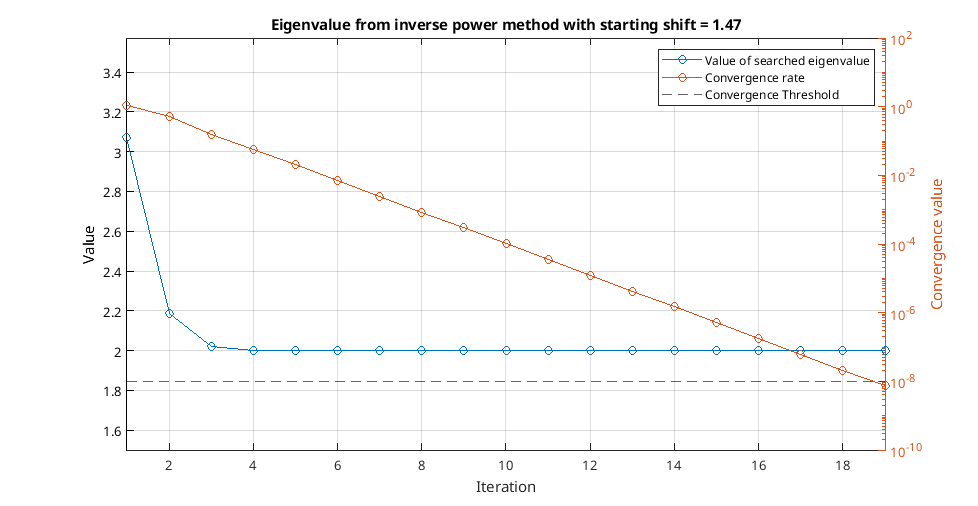
\includegraphics[width=1\textwidth]{problems/Figures/Problem2InversePowerMethod.png}
    \caption{Eigenvalue approximation and convergence rate over each iteration of inverse power method.}
    \label{fig:Inverse}
\end{figure}
% https://tobydriscoll.net/fnc-julia/krylov/inviter.html
% https://www.netlib.org/utk/people/JackDongarra/etemplates/node96.html

\subsection{Problem 3}%
\label{sec:problem_3}
The yield $y$ of wheat in quintals per hectare appears to be a linear function of the
number of days $x_1$ of sunshine, the number of centimeters $x_2$ of rainfall, and the
number of kilograms $x_3$ of fertilizer per hectare. Find the best fit to the data in
the table with an equation in the form: $y=a_0+a_1x_1+a_2x_2+a_3x_3$.

\begin{center}
\begin{tabular}{|c|c|c|c|}
  \hline
  $y$ & $x_1$ & $x_2$ & $x_3$ \\
  \hline
  28 & 50 & 18 & 10 \\
  \hline
  30 & 40 & 20 & 16 \\
  \hline
  21 & 35 & 14 & 10 \\
  \hline
  23 & 40 & 12 & 12 \\
  \hline
  23 & 30 & 16 & 14 \\
  \hline
\end{tabular}
\end{center}

%%%%%%%%%%%%%%%%%%%%%%%%%%%%%%%%%%%%%%%%%%%%%%%%%%%%%%%%%%%%%%%%%%%%%%%%%%%%%%%
\subsubsection*{Mathematics}
%%%%%%%%%%%%%%%%%%%%%%%%%%%%%%%%%%%%%%%%%%%%%%%%%%%%%%%%%%%%%%%%%%%%%%%%%%%%%%%
\todo[inline]{Develop math description}
%%%%%%%%%%%%%%%%%%%%%%%%%%%%%%%%%%%%%%%%%%%%%%%%%%%%%%%%%%%%%%%%%%%%%%%%%%%%%%%
\subsubsection*{Solution}
%%%%%%%%%%%%%%%%%%%%%%%%%%%%%%%%%%%%%%%%%%%%%%%%%%%%%%%%%%%%%%%%%%%%%%%%%%%%%%%

\subsection{Problem 4}%
\label{sec:problem_4}
Using least squares find the ``best'' straight-line fit and the error estimates for the
slope and intercept of that line for the following set of data:
\begin{center}
  \begin{tabular}{|c|c|c|c|c|c|c|c|c|}
    \hline
    $x_i$ & 1 & 2 & 3 & 4 & 5 & 6 & 7 & 8 \\
    \hline
    $y_i$ & 1.5 & 2.0 & 2.8 & 4.1 & 4.9 & 6.3 & 5.0 & 11.5 \\
    \hline
  \end{tabular}
\end{center}
%%%%%%%%%%%%%%%%%%%%%%%%%%%%%%%%%%%%%%%%%%%%%%%%%%%%%%%%%%%%%%%%%%%%%%%%%%%%%%%
\subsubsection*{Mathematics}
%%%%%%%%%%%%%%%%%%%%%%%%%%%%%%%%%%%%%%%%%%%%%%%%%%%%%%%%%%%%%%%%%%%%%%%%%%%%%%%
We want to fit the data above to the function in the form $y = a_0 + a_1x$.
We may proceed with this problem just as in the previous ones.
\todo[inline]{Write something about the linear regression}
%%%%%%%%%%%%%%%%%%%%%%%%%%%%%%%%%%%%%%%%%%%%%%%%%%%%%%%%%%%%%%%%%%%%%%%%%%%%%%%
\subsubsection*{Solution}
%%%%%%%%%%%%%%%%%%%%%%%%%%%%%%%%%%%%%%%%%%%%%%%%%%%%%%%%%%%%%%%%%%%%%%%%%%%%%%%

\subsection{Problem 5}
Find $\mathbf{A^{-1}}$ to:

\begin{equation*}
    \matr{A} = 
    \begin{bmatrix}
        2 & 1 & 2 \\
        1 & 2 & 3 \\
        4 & 1 & 2 
    \end{bmatrix}
\end{equation*}

solving the system $\mathbf{AX=I_{3}}$.

\subsubsection*{Solution}
\lstinputlisting[style=Matlab-editor]{problems/Problem_5.m}
which judges well our algorithms.

\subsection{Problem 6}

Apply the LU factorization to the matrix
\begin{equation*}
    \matr{A} = 
    \begin{bmatrix}
        \phantom{-}1 & 2 & 3 & 4 \\
        -1 & 1 & 2 & 1 \\
        \phantom{-}0 & 2 & 1 & 3 \\
        \phantom{-}0 & 0 & 1 & 1
    \end{bmatrix}
\end{equation*}
Then calculate $\det(\matr{A})$ using the matrix $\matr{U}$. Finally solve $\matr{A}\matr{x}=\matr{b}$ for $\matr{b}=[1\dots1]^T$.
\subsubsection*{Mathematics}
The LU Factorization decomposes matrix $\matr{A}$ into an upper triangular matrix $\matr{U}$ and unit lower triangular matrix $\matr{L}$, so that
\begin{equation*}
    \matr{A} = \matr{L}\matr{U}
\end{equation*}
Using the property of a determinant and a fact, that $\det(\matr{L}) = 1$ one can calculate $\det(\matr{A})$ as
\begin{equation*}
    \det(\matr{A}) = \det(\matr{L}\matr{U}) = \det(\matr{L}) \cdot \det(\matr{U}) = \det(\matr{U}) = u_{11}\cdots u_{nn}
\end{equation*}
\subsubsection*{Solution}
A glance at the matrix $\matr{A}$ tells us that it is not strictly diagonally dominant, so a pivoting algorithm should be used.
%\footnote{$\matr{A}\in\mathbb{R}^{n\times n}$ is \textit{strictly diagonally dominant} if $|a_{ii}|>\sum_{j=1 j i}^n|a_{ij}|$}
\lstinputlisting[style=Matlab-editor]{problems/Problem_6.m}

\subsection{Problem 11}%
\label{sec:problem_11}
Generate the values of the polynomial $y = 40 + 10x + 5x^2 + 3x^3 + 2x^4 + x^5 + x^6$
for $x = 1, 2, \ldots, 14$.
First fit the polynomial $y = a_0 + a_1x + a_2x^2 + a_3x^3 + a_4x^4 + a_5x^5 + a_6x^6$
to the generated data in the LS sense and compare the estimated coefficients
$a_0, a_1, \ldots, a_6$ to the true ones.
Then perturb the observed data with an additive Gaussian noise $\it{N}(0,\sigma^2)$, and
illustrate the fitting error (the Euclidean norm) versus the standard deviation $\sigma$.
Estimate the maximal value of $\sigma$ for which fitting error does not exceed $10^{-6}$,
assuming double precision arithmetic operations.
%%%%%%%%%%%%%%%%%%%%%%%%%%%%%%%%%%%%%%%%%%%%%%%%%%%%%%%%%%%%%%%%%%%%%%%%%%%%%%%

%%%%%%%%%%%%%%%%%%%%%%%%%%%%%%%%%%%%%%%%%%%%%%%%%%%%%%%%%%%%%%%%%%%%%%%%%%%%%%% Recursive Least Squares

\subsubsection*{Exponentially Weighted Recursive Least Squares}
\begin{enumerate}
    \item \textbf{Parameter Vector Initialization:}
    \[ \hat{\theta} = \mathbf{0} \]
    where \( \hat{\theta} \) is the estimate of the parameter vector of length \texttt{param\_num}.
    
    \item \textbf{Error Covariance Matrix Initialization:}
    \[ P = 1000 \cdot I \]
    where \( I \) is the identity matrix of size \texttt{param\_num} $\times$ \texttt{param\_num}. This large initial value indicates high uncertainty in the initial parameter estimates.
    
    \item \textbf{Forgetting Factor:}
    \[ \lambda = 0.99 \]
    a value close to 1, indicating that recent observations are slightly more weighted than older ones.
\end{enumerate}

\subsubsection*{Recursive Update For Each Observation}

For each observation at time step \(i\), the algorithm updates the estimate of \( \hat{\theta} \) as follows:

\begin{enumerate}
    \setcounter{enumi}{4}
    \item \textbf{Regression Vector Construction:}
    The regression vector \( \phi_i \) is constructed for each observation, with \( \phi_{i,j} = x_i^{j-1} \) for \( j = 1, \ldots, \text{param\_num} \).
    
    \item \textbf{Error Covariance Matrix Update:}
    \[ P = \left( P - \frac{P \phi_i \phi_i^T P}{\lambda + \phi_i^T P \phi_i} \right) / \lambda \]
    
    \item \textbf{Kalman Gain Calculation:}
    \[ K = P \phi_i \]
    
    \item \textbf{Parameter Estimate Update:}
    \[ \hat{\theta} = \hat{\theta} + K \left( y_i - \phi_i^T \hat{\theta} \right) \]
\end{enumerate}

\subsubsection*{Mathematical Representation}

Used Exponentially Weighted Recursive Least Squares algorithm is represented as follows:

\begin{enumerate}
    \item Initialize:
    \[ \hat{\theta} = \mathbf{0}, \quad P = 1000 \cdot I, \quad \lambda = 0.99 \]
    
    \item For each observation \(i\) from 1 to \(n\):
    \begin{itemize}
        \item[a.] Construct \( \phi_i \) with \( \phi_{i,j} = x_i^{j-1} \).
        \item[b.] Update \( P \):
        \[ P = \left( P - \frac{P \phi_i \phi_i^T P}{\lambda + \phi_i^T P \phi_i} \right) / \lambda \]
        
        \item[c.] Compute \( K \):
        \[ K = P \phi_i \]
        
        \item[d.] Update \( \hat{\theta} \):
        \[ \hat{\theta} = \hat{\theta} + K \left( y_i - \phi_i^T \hat{\theta} \right) \]
    \end{itemize}
\end{enumerate}

This algorithm recursively updates the parameter estimates \( \hat{\theta} \) based on new observations \( (x_i, y_i) \), adjusting the estimate to minimize the error between the model predictions and the observed data. The key feature of RLS is its ability to adapt the estimates as new data arrives, with the forgetting factor \( \lambda \) moderating the influence of older observations on the current estimate.

\subsubsection*{Mathematics}
\subsubsection*{Calculating $\sigma$ for given fitting error}
To analytically find $\sigma$ value for defined fitting error of $10^{-6}$, first would be redefinition of our regression model
\[
    y = a_0 + a_1 x + a_2 x^2 + a_3 x^3 + a_4 x^4 + a_5 x^5 + a_6 x^6 + \epsilon
\]
where \(\epsilon\) is the term denoting Gaussian noise \(N(0, \sigma^2)\).\\
In next step the design matrix \(A\) for the polynomial regression, which includes terms for \(x, x^2, \ldots, x^6\).\\
With observed points in \(x = 1, 2, \ldots, 14\), this matrix becomes a Vandermonde matrix.\\
The least squares estimation of the coefficients, \(\hat{a}\), in matrix form is given by:
\[
    \hat{a} = (A^T A)^{-1} A^T b
\]
The influence of noise \(\epsilon\) on the estimation is reflected in the covariance matrix which is under the influence of noise \(\epsilon\) is:
\[
    \text{Cov}(\hat{a}) = \sigma^2 (A^T A)^{-1}
\]
Each element of this matrix represents the variance of the corresponding coefficient due to noise.

\textbf{Objective:}
Solve for \(\sigma\) such that the Euclidean norm of the difference between the original coefficients and those estimated from noisy data equals \(10^{-6}\). Formally:
\[
    \sqrt{\sum_{i=0}^6 (a_i - \hat{a}_i)^2} = 10^{-6}
\]

\subsubsection*{Calculation Steps}
Each coefficient's variance can be extracted from the covariance matrix:
\[
    \text{Var}(\hat{a}_i) = \sigma^2 (A^T A)^{-1}_{ii}
\]
Assuming the noise affects each coefficient independently, the sum of squared differences due to noise is:
\[
    \sum_{i=0}^6 \sigma^2 (A^T A)^{-1}_{ii} = 10^{-12}
\]
This equation arises from setting the Euclidean norm squared of the difference (the sum of squares) to \(10^{-12}\), reflecting that the total error in terms of the Euclidean norm is \(10^{-6}\).

By rearranging given equation we are able to solve for \(\sigma\):
\[
    \sigma = \sqrt{\frac{10^{-12}}{\sum_{i=0}^6 (A^T A)^{-1}_{ii}}}
\]
Denominator is the trace of \((A^T A)^{-1}\), which sums the variances across all coefficients.\\
By using MATLAB calculated $\sigma$ value is $\approx 8.86*10^{-8}$.

%%%%%%%%%%%%%%%%%%%%%%%%%%%%%%%%%%%%%%%%%%%%%%%%%%%%%%%%%%%%%%%%%%%%%%%%%%%%%%%
%%%%%%%%%%%%%%%%%%%%%%%%%%%%%%%%%%%%%%%%%%%%%%%%%%%%%%%%%%%%%%%%%%%%%%%%%%%%%%%
\subsubsection*{Solution}
Generated curves for approximations of polynomial 
\begin{figure}[H]
    \centering
    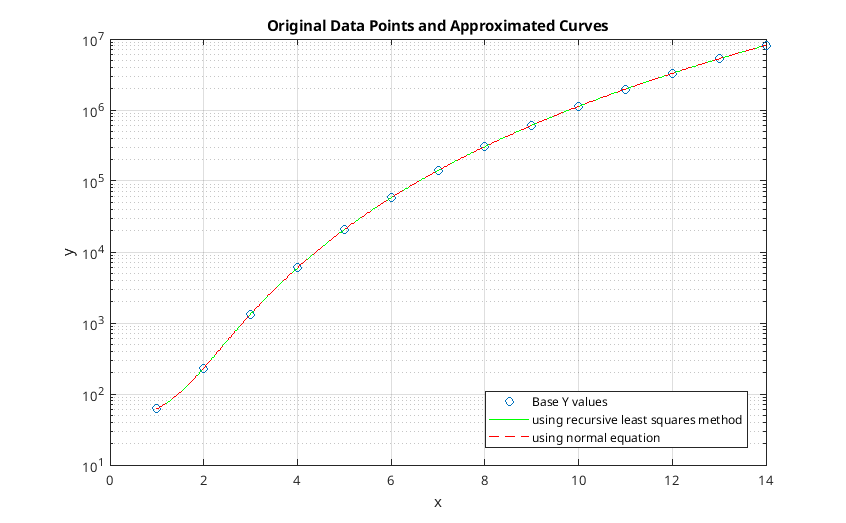
\includegraphics[width=1\textwidth]{images/Problem_11/ApproxCurves.png}
    \caption{Approximations of polynomial using Normal equation and Recursive Least Squares method}
\end{figure}
During the programming of fitting error calculation, we weren't able to get such low values for fitting error. 
It's possible that our method for calculating fitting error was incorrect, or used methods had awful stability.
For $\sigma \in (0:0.0001:0.1)$ our lowest error was with the use of normal equation at $1.0953*10^-5$.
\begin{figure}[H]
    \centering
    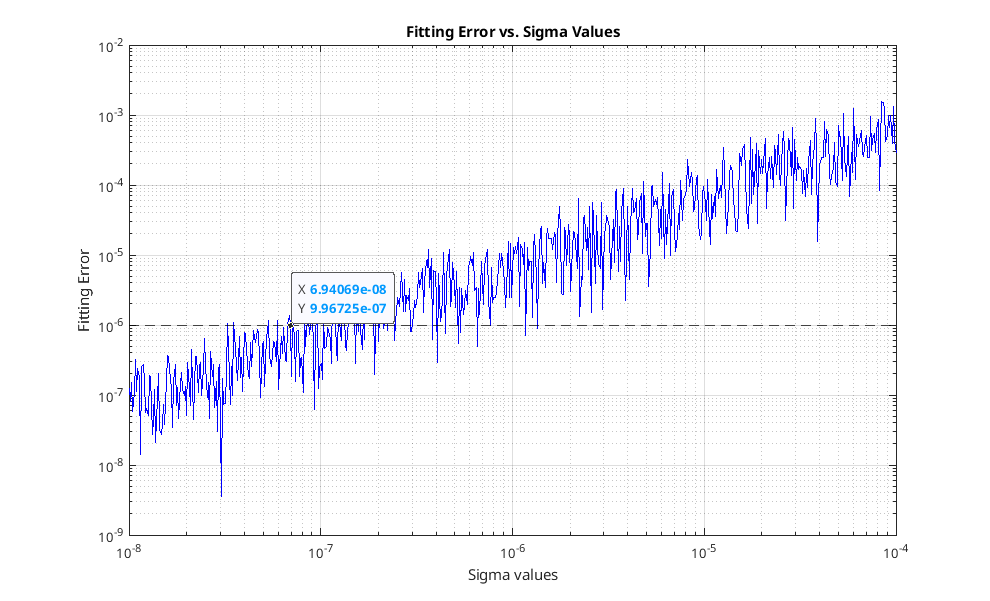
\includegraphics[width=1\textwidth]{images/Problem_11/fittingErrors.png}
    \caption{Fitting errors of approximations Normal equation and RLS with perturbed input data set}
\end{figure}
Weighted recursive least squares method had higher fitting error than normal equation.
%%%%%%%%%%%%%%%%%%%%%%%%%%%%%%%%%%%%%%%%%%%%%%%%%%%%%%%%%%%%%%%%%%%%%%%%%%%%%%%


\clearpage

\section{Algorithms}
\subsection{Algorithm~1: Normal equations approximation}%
\label{algorithm:1}
\lstinputlisting[style=Matlab-editor, breaklines=false]{algorithms/normal_approximation.m}

%%%%%%%%%%%%%%%%%%%
%% BIBLIOGRAPHY %%%
%%%%%%%%%%%%%%%%%%%

\clearpage

\nocite{Zdunek, GoluVanl96, Meyer}
\bibliographystyle{alpha}
\bibliography{bibliography}

\end{document}
